\clearpage
\section{Paramétrage de SimFeodal}
	
\subsection{Avant propos sur le paramétrage d'un modèle complexe}
	
	\todobox{
	A changer : le chap 2 présentera la version 0 (Base) du modèle, et on vient donc ici montrer comment on a répondu aux limites identifiées à la fin du chapitre, cf. les conclusions/résultats du chapitre TransMonDyn.
	}
\medbreak
	
	\todobox{
	Pour introduire le schéma des étapes, rappeler ici que les paramètres et mécanismes d'un modèle complexe sont en interaction, ce qui produit des effets non linéaires.\\
	Principe des vases communicants !\\
	Mentionner aussi la logique des attracteurs étranges de Lorenz comme paroxysme de cette complexité : ici, moins de variation, mais des répercussions importantes tout de même qu'il faut donc \og corriger\fg{} par de nombreuses itérations de modifications.
	}

Le tableau suivant (\cref{table:etapes-construction}) se veut être un point de repère autant qu'une table des matières synthétique pour la compréhension des étapes qui suivent. Si la description de chacune de celles-ci revêt une forme assez factuelle et systématique, nous pensons toutefois que l'explicitation de chacune de ces étapes permet de saisir la démarche proposée ainsi que l'intérêt de celle-ci.

Notons que l'étape 0 ici présentée correspond à une première version \og exploitable\fg{} du modèle, c'est-à-dire contenant \textit{a minima} l'ensemble des agents et mécanismes identifiés dans un premier temps par l'équipe de modélisation \autocite{tannier_ontologie_2014}. Nous ne détaillerons pas ici les différentes phases de construction précédentes. Nous reviendrons toutefois sur plusieurs d'entre elles, en guise d'exemples illustratifs, dans les chapitres 6 et 7 \hl{(Partie 3)}.

\subsubsection{De manière générale}
	
\subsection{Les étapes du paramètrage de SimFeodal}
	
Comme préconisé ci-dessus, le modèle SimFeodal a été paramétré tout au long de sa construction. Dans cette partie, nous reviendrons en détail sur chacune des étapes de ce paramétrage, en retraçant les choix et questionnements qui ont orienté ces modifications du modèle. L'énumération est en ordre chronologique, et l'on a essayé d'organiser ces étapes en grands blocs-type de paramétrisation. Pour autant, le paramétrage et la construction d'un modèle, et du notre en particulier, sont un travail constant d'allers-retours entre l'identification et la résolution de problèmes. La structure réelle de développement, que l'on peut retrouver dans l'historique des modifications du modèle (les \og \textit{commits}\fg{}), ne correspond donc pas exactement à la chronologie organisée qui suit.
	
	
\pagebreak
\begin{footnotesize}
	\begin{longtable}{ m{.05\textwidth} m{.08\textwidth}  m{.12\textwidth}  m{.65\textwidth}  m{.10\textwidth}  }
		\caption{Tableau récapitulatif des étapes de construction du modèle. Conception : C. Tannier (\fixref{Tannier 2017, HDR}) et R. Cura, 2017}\\
		\label{table:etapes-construction}\\
		Étape & Version & Type      & Modifications                                                 & Section                                                                                   \\
		\endfirsthead
		Étape & Version & Type      & Modifications                                                 & Section                                                                                   \\
		\endhead			
		\hline
		0      & Base    & Création & Création du modèle. \fixref{Cf. tableau 14 de Tannier 2017} & Chap 2\footnote{On s'appuie sur cette version \og Base\fg{} dans le \fixref{chapitre 2}.} \\
		\hline
		1 & Base2 & paramétrage & \colorbox{yellow}{Hiérarchisation} des valeurs d'attraction des attracteurs. \newline
		Modification des critères de création de nouvelles paroisses. \newline
		Réduction de la distance maximale de déplacement local. \newline
		Assouplissement des règles de promotion d'un château en gros château. & Chap3-x.y\\
		\hline
		2 & Base2 compo5 2bis & modélisation et paramétrage & Assouplissement des règles de création d'une paroisse.\newline
		Réduction de la distance maximale de déplacement local. \newline
		Modification des règles de calcul de la probabilité de construire un château.\newline
		Modification du calcul de la satisfaction matérielle des foyers paysans. & Chap3-x.y\\
		\hline
		3 & Base2 compo5 2quat & modélisation et paramétrage & \colorbox{yellow}{Hiérarchisation} des valeurs d'attraction des attracteurs. \newline
		Facilitation de la construction de châteaux. \newline
		Rationnalisation du déplacement des foyers paysans. \newline
		Ajout d'un nouveau type d'attracteur, les communautés. & Chap3-x.y\\
		\hline
		4 & Base3 2 & modélisation et paramétrage & \colorbox{yellow}{Hiérarchisation} des valeurs d'attraction des attracteurs. \newline
		Modification des critères de création de nouvelles paroisses. \newline
		Augmentation de la distance maximale de déplacement local. \newline
		Modification de la procédure d'identification des agrégats et des pôles. & Chap3-x.y\\
		\hline
		5 & Base4 1 & modélisation et paramétrage & 
		Modification de la répartition initiale des foyers paysans.\newline
		Simplification de la procédure d'identification d'héritage des agrégats.
		Amélioration de la définition des pôles d'attraction et de leur enveloppe. & Chap3-x.y\\
		\hline
		6 & Base4 2 & modélisation et paramétrage & \colorbox{yellow}{Hiérarchisation} des valeurs d'attraction des attracteurs. \newline
		Modification de l'ordonnancement des actions dans le modèle.\newline
		Modification de la procédure d'identification des agrégats. & Chap3-x.y\\
		\hline
		7 & Base4 3ter & modélisation et paramétrage &
		Dynamisation de la distance maximale de déplacement local.\newline
		Modification du calcul de satisfaction des foyers paysans. & Chap3-x.y\\
		\hline
		8 & Base4 4A & modélisation & Modification de l'ordonnancement des actions dans le modèle.\newline
		Modification du mécanisme de déplacement local des foyers paysans. & Chap3-x.y\\
		\hline
					
	\end{longtable}
\end{footnotesize}

%\subsubsection{Étape 0}
%	
%\paragraph{Indicateurs généraux}
%	
%\begin{table}[H]
%	\centering
%	\caption{Indicateurs synthétiques de l'étape 1}
%	\label{my-label}
%	\begin{tabular}{lll}
%		Indice             & Objectif & Moyenne \\
%		Nb agrégats       & 200.00   & 145.30  \\
%		Nb châteaux       & 50.00    & 69.78   \\
%		Nb gros  Châteaux & 10.00    & 9.60    \\
%		Nb egl. Par.       & 300.00   & 167.90  \\
%		Dist entre égl.   & 3000.00  & 2944.00 \\
%		FP isolés         & 0.20     & 0.49    \\
%		Ratio Charge Fisc. & 3.00     & 5.15    
%	\end{tabular}
%\end{table}
%
%\pagebreak
%\subsubsection{Étape 1}
%\begin{figure}[H]
%	\centering
%	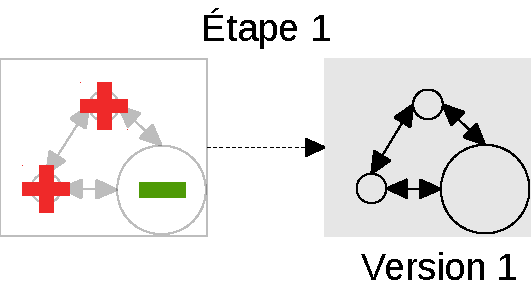
\includegraphics[width = \linewidth, page = 1]{img/schemas_etapes_individuelles.pdf}
%	\caption{Étape 1 du paramétrage et résultats.}
%\end{figure}
%
%\pagebreak
%\subsubsection{Étape 2}
%\begin{figure}[H]
%	\centering
%	\includegraphics[width = \linewidth, page = 2]{img/schemas_etapes_individuelles.pdf}
%	\caption{Étape 2 du paramétrage et résultats.}
%\end{figure}
%
%\pagebreak
%\subsubsection{Étape 3}
%\begin{figure}[H]
%	\centering
%	\includegraphics[width = \linewidth, page = 3]{img/schemas_etapes_individuelles.pdf}
%	\caption{Étape 3 du paramétrage et résultats.}
%\end{figure}
%
%\pagebreak
%\subsubsection{Étape 4}
%\begin{figure}[H]
%	\centering
%	\includegraphics[width = \linewidth, page = 4]{img/schemas_etapes_individuelles.pdf}
%	\caption{Étape 4 du paramétrage et résultats.}
%\end{figure}
%
%\pagebreak
%\subsubsection{Étape 5}
%\begin{figure}[H]
%	\centering
%	\includegraphics[width = \linewidth, page = 5]{img/schemas_etapes_individuelles.pdf}
%	\caption{Étape 5 du paramétrage et résultats.}
%\end{figure}
%
%\pagebreak
%\subsubsection{Étape 6}
%\begin{figure}[H]
%	\centering
%	\includegraphics[width = \linewidth, page = 6]{img/schemas_etapes_individuelles.pdf}
%	\caption{Étape 6 du paramétrage et résultats.}
%\end{figure}
%
%\pagebreak
%\subsubsection{Étape 7}
%\begin{figure}[H]
%	\centering
%	\includegraphics[width = \linewidth, page = 7]{img/schemas_etapes_individuelles.pdf}
%	\caption{Étape 7 du paramétrage et résultats.}
%\end{figure}
%
%\pagebreak
%\subsubsection{Étape 8}
%\begin{figure}[H]
%	\centering
%	\includegraphics[width = \linewidth, page = 8]{img/schemas_etapes_individuelles.pdf}
%	\caption{Étape 8 du paramétrage et résultats.}
%\end{figure}
%	
%\pagebreak
\subsection{Un bilan des changements majeurs à l'issu du paramétrage}
	
\begin{figure}[H]
	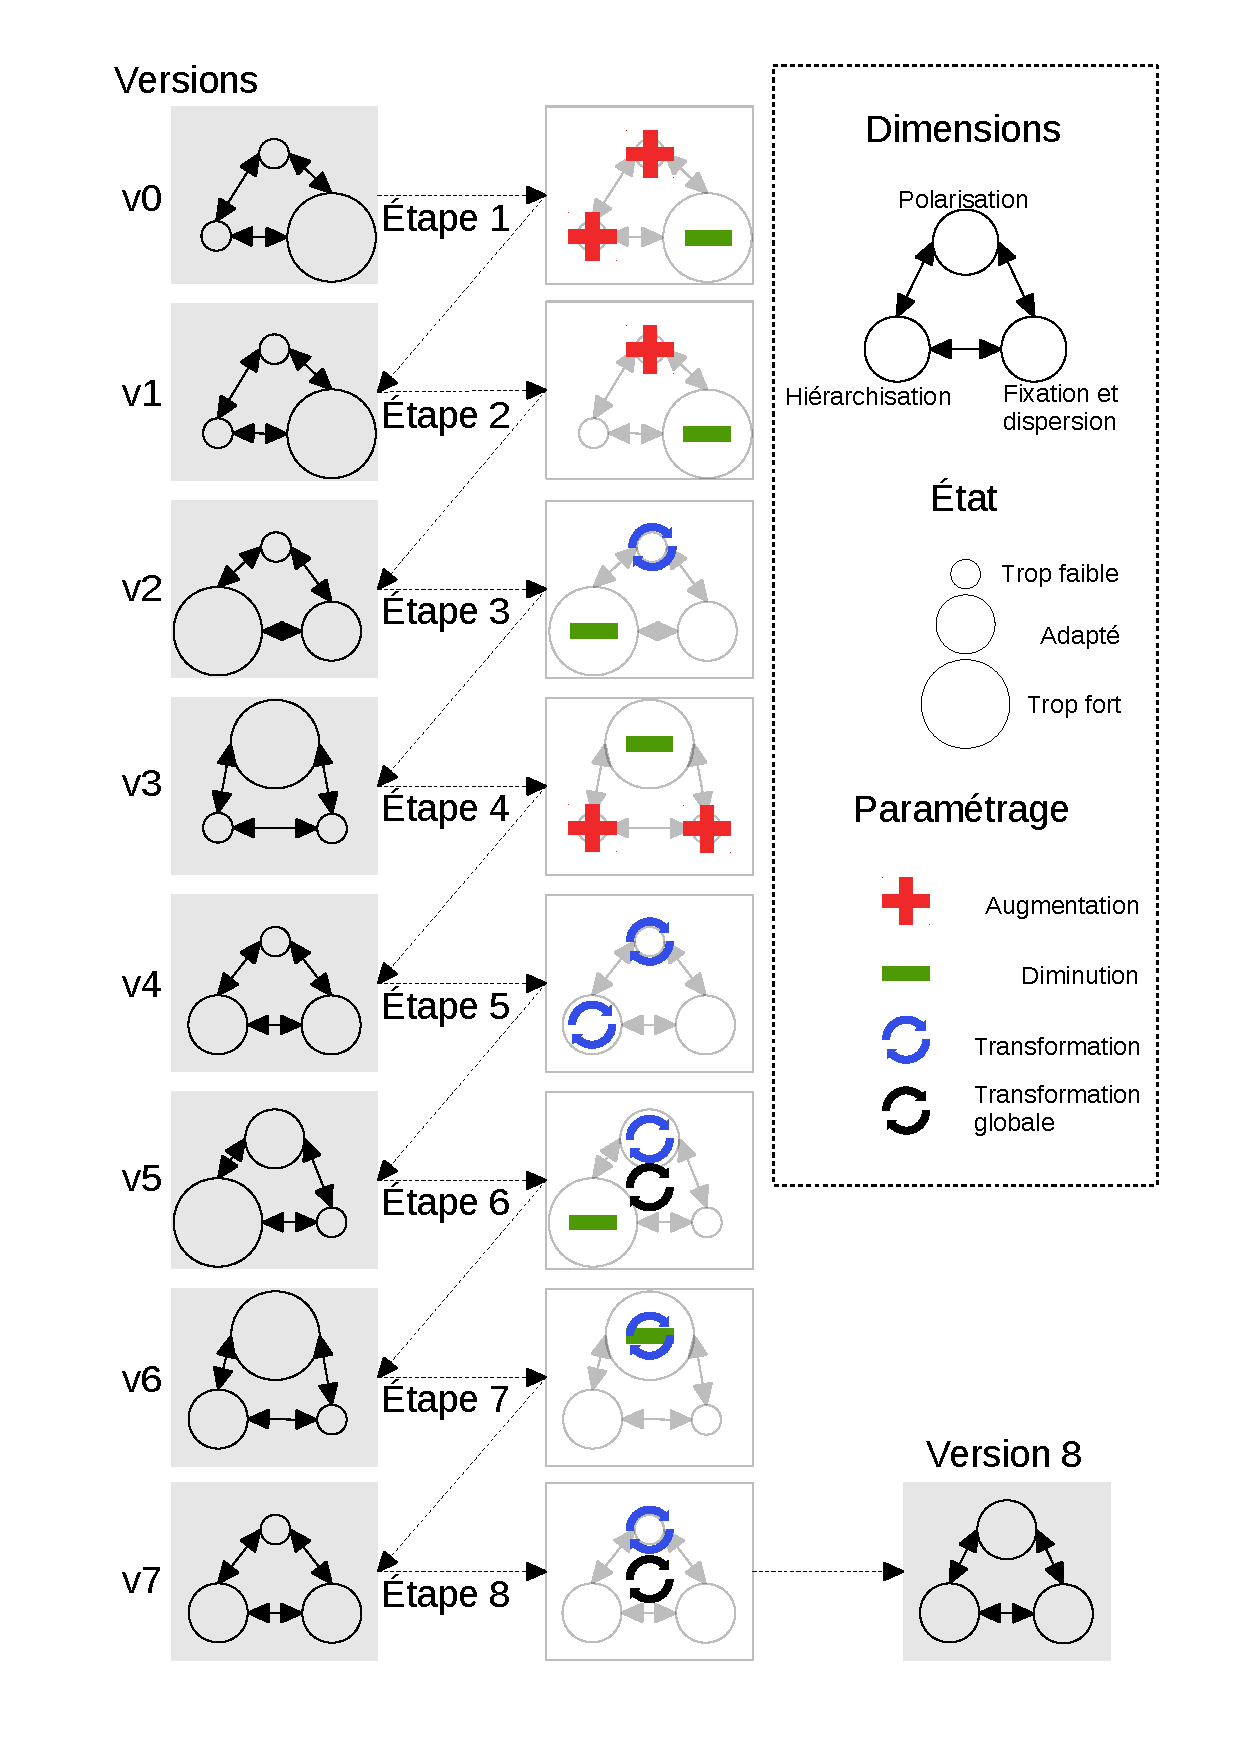
\includegraphics[width = \linewidth, page = 1]{img/schema_etapes_complet.pdf}
	\caption{Schéma récapitulatif et synthétique des étapes du paramétrage de SimFeodal.}
	\label{fig:etapes-parametrage-simfeodal}
\end{figure}
	